\documentclass[article]{jss}
\usepackage[utf8]{inputenc}

\providecommand{\tightlist}{%
  \setlength{\itemsep}{0pt}\setlength{\parskip}{0pt}}

\author{
John Muschelli\\Department of Biostatistics, Johns Hopkins Bloomberg School of Public
Health
}
\title{ROC and AUC with a Binary Predictor}

\Plainauthor{John Muschelli}
\Plaintitle{ROC and AUC with a Binary Predictor}
\Shorttitle{Binary Predictor ROC}

\Abstract{
The abstract of the article.
}

\Keywords{roc, auc, area under the curve, \proglang{R}}
\Plainkeywords{roc, auc, area under the curve, R}

%% publication information
%% \Volume{50}
%% \Issue{9}
%% \Month{June}
%% \Year{2012}
%% \Submitdate{}
%% \Acceptdate{2012-06-04}

\Address{
    John Muschelli\\
  Department of Biostatistics, Johns Hopkins Bloomberg School of Public
  Health\\
  615 N Wolfe St Baltimore, MD 21205\\
  E-mail: \email{jmuschel@jhsph.edu}\\
  URL: \url{http://johnmuschelli.com}\\~\\
  }

% Pandoc header

\usepackage{amsmath}

\begin{document}

\hypertarget{introduction}{%
\section{Introduction}\label{introduction}}

In many applications, receiver operator characteristic (ROC) curves are
used to show how a predictor compares to the true outcome. One of the
large advantages of ROC analysis is that it is threshold-agnostic; it
shows the performance of a predictor without a specific threshold and
also gives a criteria to choose an optimal threshold based on a certain
cost function. Typically, an ROC analysis shows how sensitivity changes
with varying specificity.

Many predictors, especially medical tests, result in a binary decision;
a value is higher than a pre-determined threshold or not. Similarly,
some are simply categorical or discrete; for example, blood pressure may
be low, normal, or high. These are useful indicators of presence
disease, which is a primary outcome of interest. The predictive
capabilities of the variable is summarized many times in the area under
the curve (AUC). Additionally, partial ROC (pROC) analysis keeps a
specificity fixed and determines the optimal sensitivity or the partial
AUC (pAUC).

One can assume the binary predictor is generated from a continuous
distribution that has been thresholded. Therefore, the sensitivity of
this thresholded predictor actually represents one point on the ROC
curve of the true underlying continuous distribution. Therefore the ROC
curve of a binary predictor is not really appropriate, but should be
represented by a single point on the curve. But alas, ROC and AUC
analysis is done on binary predictors and used to inform if one variable
is more predictive than the other \citep[\citet{jama2}]{jama}. For
example, these cases

A more appropriate comparison of a continuous predictor and the binary
predictor may be to compare the sensitivity and specificity (or overall
accuracy) of the continuous predictor given the optimal threshold versus
that of the binary predictor.

\citet{fawcett2006introduction} describes (in Fig. 6) how ties are
handled in a predictor. Ties are distinctly relevant for discrete and
binary predictors or models that predict a discrete number of values,
where many observations can have the same value/risk score. When drawing
the ROC curve, one can assume that all the ties do not correctly
classify the outcome (Fawcett called the ``pessimistic'' approach) or
that all the ties do correclty classify the outcome (called the
``optimistic'' approach). But Fawcett notes:

\begin{quote}
Any mixed ordering of the instances will give a different set of step
segments within the rectangle formed by these two extremes. However, the
ROC curve should represent the \emph{expected} performance of the
classifier, which, lacking any other information, is the average of the
pessimistic and optimistic segments.
\end{quote}

This ``expected'' performance directly applies to the assignment of a
half probability of success when the data are tied, which is implied by
the ``trapezoidal rule'' from \citet{hanley1982meaning}. This half
probability is linked to how ties are treated in the Wilcoxon rank sum
test. As much of the theory of ROC curve testing, and therefore testing
of differences in AUC, is based on the theory of the Wilcoxon rank-sum
test, this treatment of ties is relevant to statistical inference.

We show the commonly used software for calculating AUC may be misleading
for binary or categorical predictors depending on the definition of the
AUC.

\hypertarget{mathematical-proof-of-auc-for-single-binary-predictor}{%
\section{Mathematical Proof of AUC for Single Binary
Predictor}\label{mathematical-proof-of-auc-for-single-binary-predictor}}

Let us assume we have a binary predictor \(X\) and a binary outcome
\(Y\), such that \(X\) and \(Y\) only take the values \(0\) and 1. Let
\(X_{i}\) be the values of \(X | Y = i\), where \(i \in \{0, 1\}\).

Fawcett goes on to state: \textgreater{} AUC of a classifier is
equivalent to the probability that the classifier will rank a randomly
chosen positive instance higher than a randomly chosen negative
instance.

In other words, we \(\text{AUC} = P(X_{1} > X_{0})\). As there are only
two outcomes for \(X\), we can expand this probability using the law of
total probability:

\begin{align}
P(X_{1} > X_{0}) &= P(X_{1} > X_{0} | X_{1} = 1) P(X_{1} = 1) \nonumber \\
&+ P(X_{1} > X_{0} | X_{1} = 0) P(X_{1} = 0) \label{eq:expand1} \\
&= P(X_{1} > X_{0} | X_{1} = 1) P(X_{1} = 1) \label{eq:expand}
\end{align}

as \(P(X_{1} > X_{0} | X_{1} = 0) = 0\) because \(X_{0} \in \{0, 1\}\).
We see that \(P(X_{1} = 1)\) in equation \eqref{eq:expand} is the
sensitivity:

\begin{align*}
P(X_{1} = 1) &= P(X = 1 | Y = 1)\\
&= \frac{TP}{TP + FN} \\
&= \text{sensitivity}
\end{align*}

and that \(P(X_{1} > X_{0} | X_{1} = 1)\) in equation \eqref{eq:expand}
is the specificity:

\begin{align*}
P(X_{1} > X_{0} | X_{1} = 1) &= P(X_{1} > X_{0} | X_{1} = 1, X_{0} =1) P(X_{0} = 1) \\
&+ P(X_{1} > X_{0} | X_{1} = 1, X_{0} =0) P(X_{0} = 0) \\
&= P(X_{1} > X_{0} | X_{1} = 1, X_{0} =0) P(X_{0} = 0) \\
&= P(X_{0} = 0) \\
&= P(X = 0 | Y = 0)\\
&= \frac{TN}{TN + FP} \\
&= \text{specificity}
\end{align*}

Therefore, we combine these two to show that equation \eqref{eq:expand}
reduces to:

\[
P(X_{1} > X_{0}) = \text{specificity} \times \text{sensitivity}
\]

\hypertarget{simple-example}{%
\subsection{Simple Example}\label{simple-example}}

Let's assume \(X\) and \(Y\) have the following joint distribution:

\begin{tabular}{l|r|r}
\hline
  & 0 & 1\\
\hline
0 & 52 & 35\\
\hline
1 & 32 & 50\\
\hline
\end{tabular}

Therefore, the AUC should be equal to
\(\frac{50}{85} \times \frac{52}{84}\), which equals:

\begin{CodeChunk}

\begin{CodeOutput}
[1] 0.3641457
\end{CodeOutput}
\end{CodeChunk}

As this is the strict definition of AUC, let us call this
\(\text{AUC}_{\text{definition}}\).

Note, if we reverse the labels, then the sensitivity and the specificity
are estimated by \(1\) minus that measure, or
\(\frac{35}{85} \times \frac{32}{84}\), which is equal to:

\begin{CodeChunk}

\begin{CodeInput}
R> flip.auc = (1 - sens) * (1 - spec)
R> print(flip.auc)
\end{CodeInput}

\begin{CodeOutput}
[1] 0.1568627
\end{CodeOutput}
\end{CodeChunk}

Thus, as this AUC is less than the original labeling, we would choose
that with the original labeling.

If we change the definition of AUC slightly while accounting for ties,
\(\text{AUC}_{\text{w/ties}}\) to \[
\text{AUC}_{\text{w/ties}} = P(X_{1} > X_{0}) + \frac{1}{2} P(X_{1} = X_{0})
\] we see that we would calculate the AUC by
\(\text{AUC}_{\text{definition}} + \frac{1}{2}\left( \frac{50 + 52}{169}\right)\),
which is equal to:

\begin{CodeChunk}

\begin{CodeOutput}
[1] 0.6036415
\end{CodeOutput}
\end{CodeChunk}

We will explore the estimated ROC curve and AUC from the implentations
in the follwing \texttt{R} packages: \pkg{ROCR} \citep{ROCR},
\pkg{caTools}, \pkg{pROC} \citep{pROC}, and \pkg{fbroc} \citep{fbroc}.
We will also show these agree with the Python implementation in
\texttt{sklearn.metrics} \citep{scikitlearn} and the Stata function
\texttt{roctab}. We note that these functions all count half the
probability of ties, which raises the AUC. We will present a geometric
discussion of the ROC as well.

\hypertarget{current-implementations}{%
\section{Current Implementations}\label{current-implementations}}

\hypertarget{r}{%
\subsection{R}\label{r}}

The \pkg{caTools} package calculates AUC using the \texttt{colAUC}
function:

\begin{CodeChunk}

\begin{CodeInput}
R> library(caTools)
R> colAUC(x, y)
\end{CodeInput}

\begin{CodeOutput}
             [,1]
0 vs. 1 0.6036415
\end{CodeOutput}
\end{CodeChunk}

In \pkg{ROCR}, AUC is calculated from a \code{performance} object, which
takes in a \code{prediction} object:

\begin{CodeChunk}

\begin{CodeInput}
R> library(ROCR)
R> yvalues = function(perf) {
R+   unlist(slot(perf, "y.values"))
R+ }
R> xvalues = function(perf) {
R+   unlist(slot(perf, "x.values"))
R+ }
R> 
R> pred = prediction(x, y)
R> auc.est = performance(pred, "auc")
R> yvalues(auc.est)
\end{CodeInput}

\begin{CodeOutput}
[1] 0.6036415
\end{CodeOutput}
\end{CodeChunk}

The \pkg{pROC} package calculates AUC using the \texttt{roc} function:

\begin{CodeChunk}

\begin{CodeInput}
R> library(pROC)
R> pROC.roc = pROC::roc(predictor = x, response = y)
R> pROC.roc[["auc"]]
\end{CodeInput}

\begin{CodeOutput}
Area under the curve: 0.6036
\end{CodeOutput}
\end{CodeChunk}

\begin{CodeChunk}


\begin{center}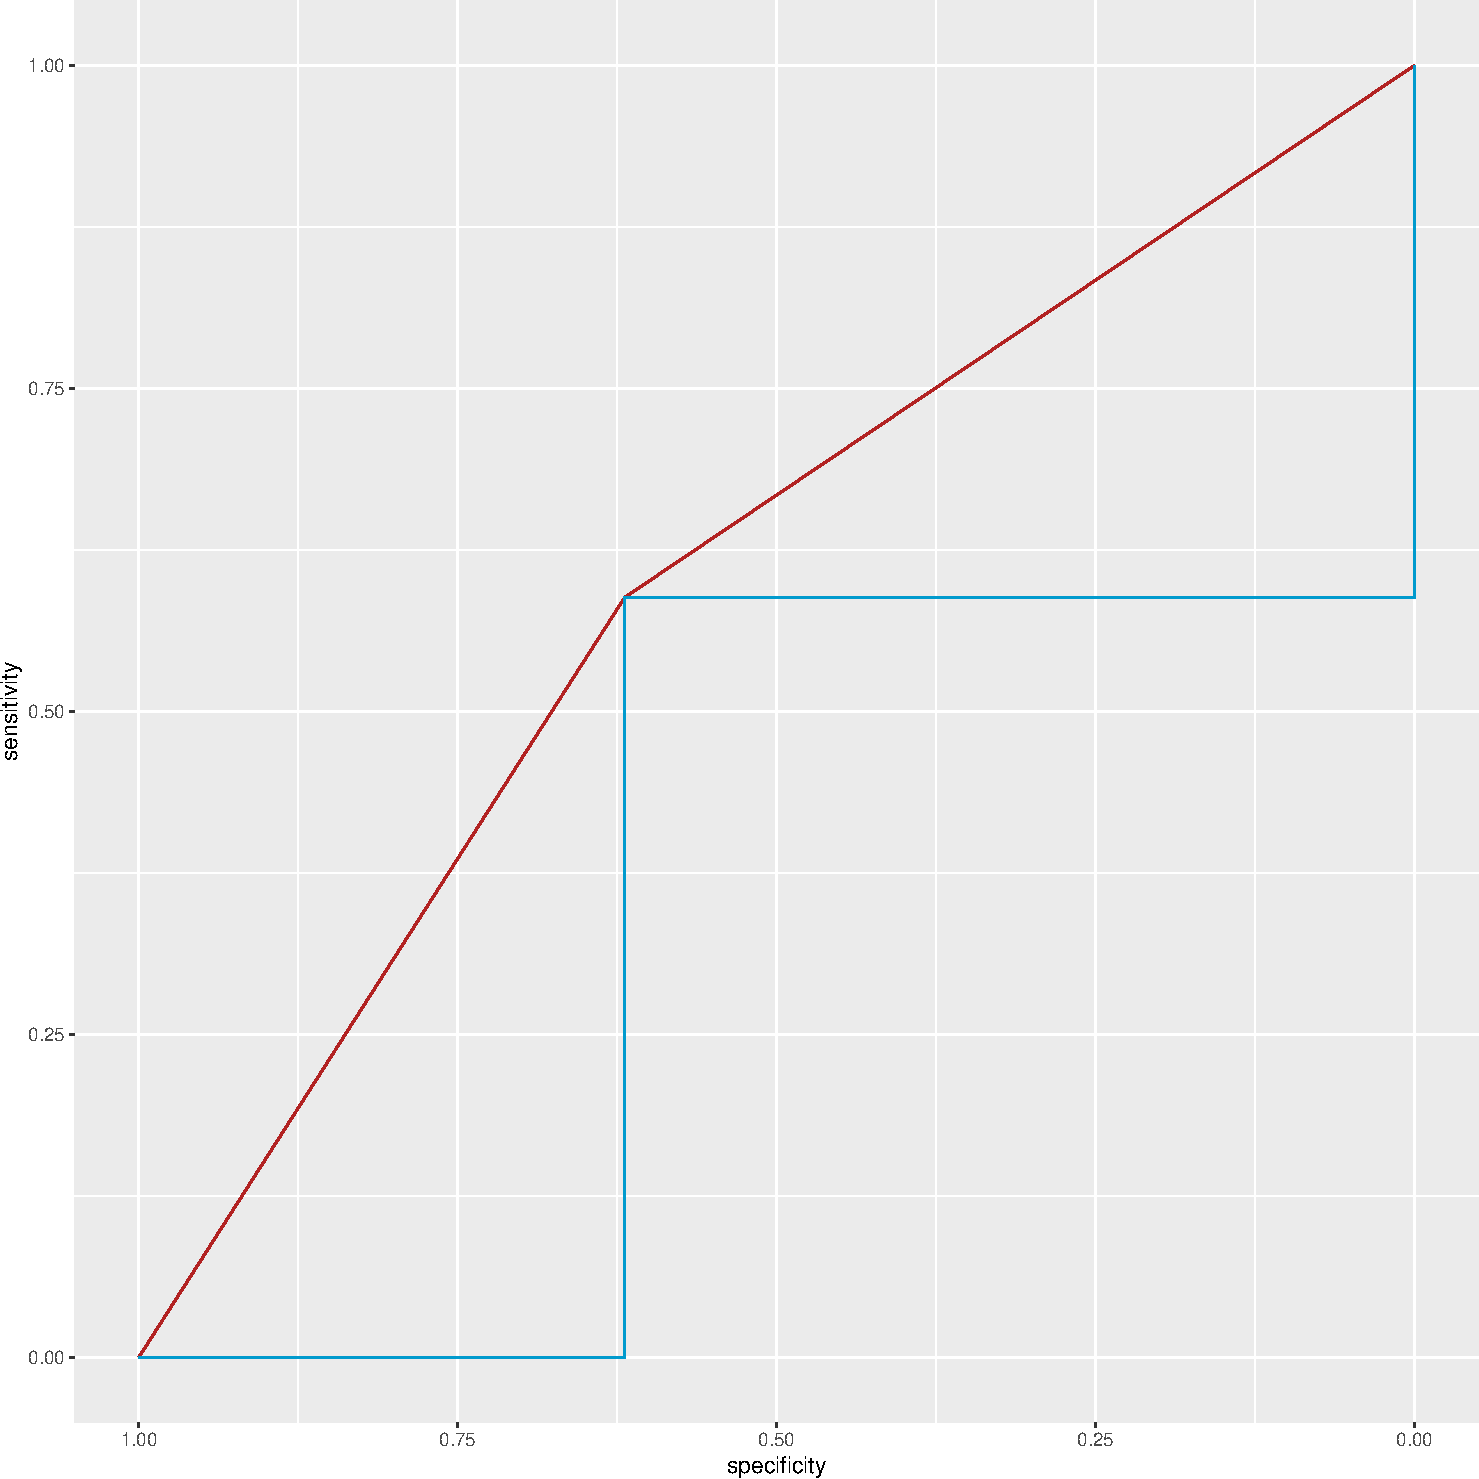
\includegraphics{index_files/figure-latex/unnamed-chunk-8-1} \end{center}

\end{CodeChunk}

\begin{CodeChunk}


\begin{center}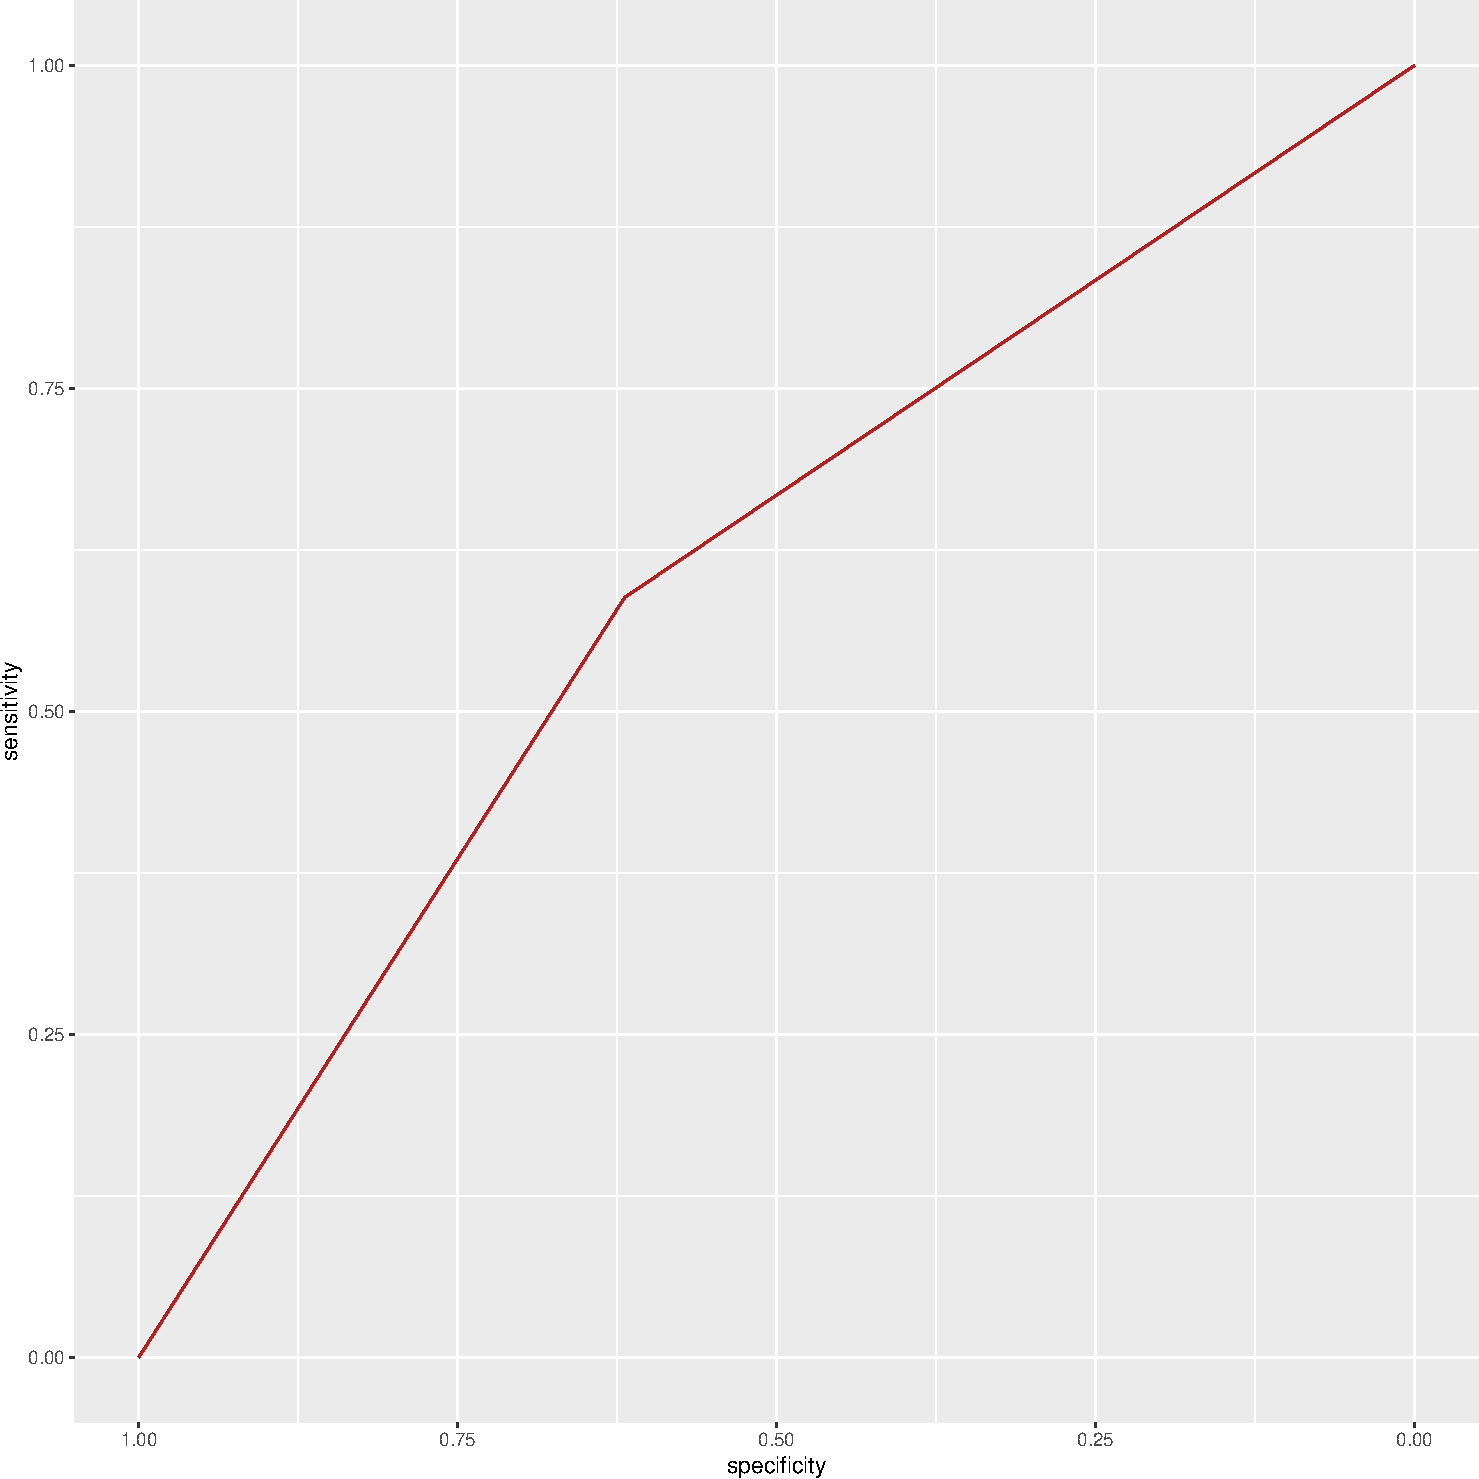
\includegraphics{index_files/figure-latex/unnamed-chunk-9-1} \end{center}

\end{CodeChunk}

Looking at the plot for the ROC curve in \pkg{ROCR}, we can see why this
may be:

\begin{CodeChunk}

\begin{CodeInput}
R> par(mfrow = c(1, 2))
R> perf = performance(pred, "tpr", "fpr")
R> plot(perf)
R> abline(a = 0, b = 1)
R> plot(perf, type = "s")
R> abline(a = 0, b = 1)
\end{CodeInput}
\end{CodeChunk}

Looking geometrically at the plot, we can see how

\begin{CodeChunk}

\begin{CodeInput}
R> fpr = 1 - spec
R> left.tri = 1/2 * sens * fpr
R> right.tri = 1/2 * spec * (1 - sens)
R> false.auc = left.tri + auc.defn + right.tri
R> false.auc
\end{CodeInput}

\begin{CodeOutput}
[1] 0.6036415
\end{CodeOutput}
\end{CodeChunk}

\hypertarget{proc-package}{%
\subsubsection{pROC Package}\label{proc-package}}

\url{http://blog.revolutionanalytics.com/2016/11/calculating-auc.html}

\hypertarget{fbroc-package}{%
\subsubsection{fbroc Package}\label{fbroc-package}}

The \pkg{fbroc} package is one of the most popular packages for doing
ROC analysis \citep{fbroc}. Using the \texttt{fbroc::boot.roc} and
\texttt{fbroc::perf} functions, we have:

\begin{CodeChunk}

\begin{CodeInput}
R> library(fbroc)
R> fbroc.default = boot.roc(x, as.logical(y), 
R+                           n.boot = 1000, tie.strategy = 2)
R> auc.def = perf(fbroc.default, "auc")
R> auc.def[["Observed.Performance"]]
\end{CodeInput}

\begin{CodeOutput}
[1] 0.6036415
\end{CodeOutput}

\begin{CodeInput}
R> fbroc.alternative = boot.roc(x, as.logical(y), n.boot = 1000, tie.strategy = 1)
R> auc.alt = perf(fbroc.alternative, "auc")
R> auc.alt[["Observed.Performance"]]
\end{CodeInput}

\begin{CodeOutput}
[1] 0.6036415
\end{CodeOutput}
\end{CodeChunk}

\textbackslash{}begin\{CodeChunk\}

\textbackslash{}begin\{CodeInput\} R\textgreater{} python\_figure =
``python\_roc.png'' R\textgreater{} \# Taken from R\textgreater{} \#
\url{https://qiita.com/bmj0114/items/460424c110a8ce22d945}
R\textgreater{} sk = import(``sklearn.metrics'') R\textgreater{} plt =
import(``matplotlib.pyplot'') R\textgreater{} py\_roc\_curve =
sk\(roc_curve(y_score = x, y_true = y) R> names(py_roc_curve) = c("fpr", "tpr", "thresholds") R> roc_auc = sk\)auc(py\_roc\_curve\(fpr, py_roc_curve\)tpr)
R\textgreater{} R\textgreater{} plt\$figure()
\textbackslash{}end\{CodeInput\}

\begin{CodeOutput}
Figure(640x480)
\end{CodeOutput}

\textbackslash{}begin\{CodeInput\} R\textgreater{}
plt\(plot(py_roc_curve\)fpr, py\_roc\_curve\$tpr, color=`darkorange',
lw=1, label= sprintf(`ROC curve (area = \%0.3f)', roc\_auc))
\textbackslash{}end\{CodeInput\}

\begin{CodeOutput}
[[1]]
Line2D(ROC curve (area = 0.604))
\end{CodeOutput}

\begin{CodeInput}
R> plt$plot(c(0, 1), c(0, 1), color='navy', lw=1, linestyle='--')
\end{CodeInput}

\begin{CodeOutput}
[[1]]
Line2D(_line1)
\end{CodeOutput}

\begin{CodeInput}
R> plt$xlim(c(0.0, 1.0))
\end{CodeInput}

\begin{CodeOutput}
[[1]]
[1] 0

[[2]]
[1] 1
\end{CodeOutput}

\begin{CodeInput}
R> plt$ylim(c(0.0, 1.05))
\end{CodeInput}

\begin{CodeOutput}
[[1]]
[1] 0

[[2]]
[1] 1.05
\end{CodeOutput}

\begin{CodeInput}
R> plt$xlabel('False Positive Rate')
\end{CodeInput}

\begin{CodeOutput}
Text(0.5,0,'False Positive Rate')
\end{CodeOutput}

\begin{CodeInput}
R> plt$ylabel('True Positive Rate')
\end{CodeInput}

\begin{CodeOutput}
Text(0,0.5,'True Positive Rate')
\end{CodeOutput}

\begin{CodeInput}
R> plt$title('Receiver operating characteristic')
\end{CodeInput}

\begin{CodeOutput}
Text(0.5,1,'Receiver operating characteristic')
\end{CodeOutput}

\textbackslash{}begin\{CodeInput\} R\textgreater{}
plt\$legend(loc=``lower right'') \textbackslash{}end\{CodeInput\}

\begin{CodeOutput}
Legend
\end{CodeOutput}

\textbackslash{}begin\{CodeInput\} R\textgreater{}
plt\$savefig(python\_figure) \textbackslash{}end\{CodeInput\}
\textbackslash{}end\{CodeChunk\}

\textbackslash{}begin\{CodeChunk\}

\textbackslash{}begin\{CodeInput\} R\textgreater{}
knitr::include\_graphics(python\_figure)
\textbackslash{}end\{CodeInput\}

\begin{center}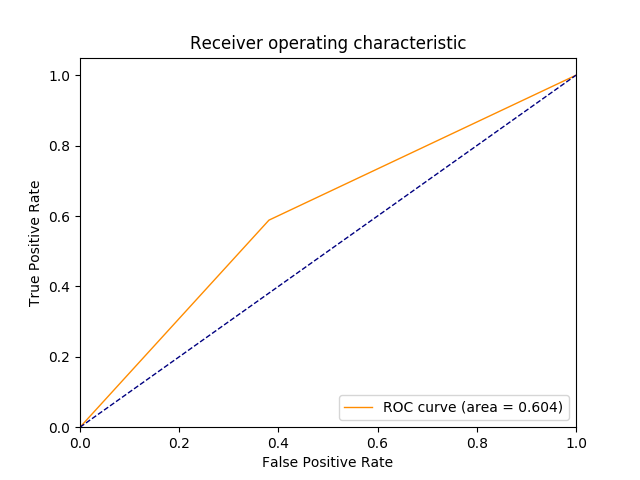
\includegraphics[width=11.11in]{python_roc} \end{center}

\textbackslash{}end\{CodeChunk\}

\begin{CodeChunk}


\begin{center}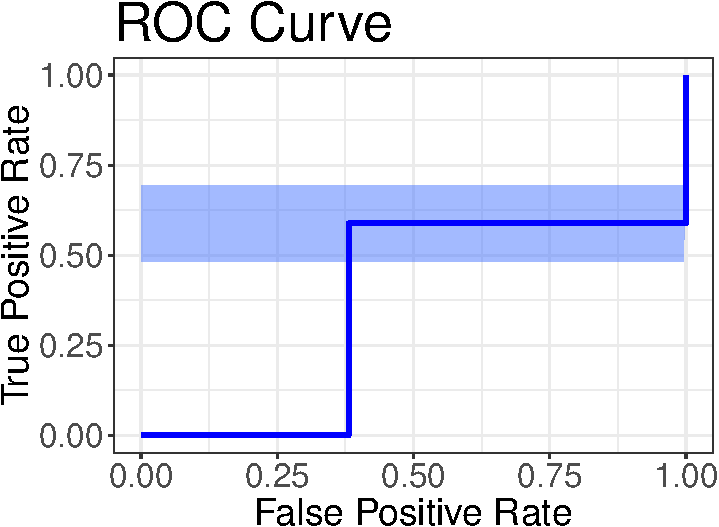
\includegraphics{index_files/figure-latex/unnamed-chunk-15-1} \end{center}



\begin{center}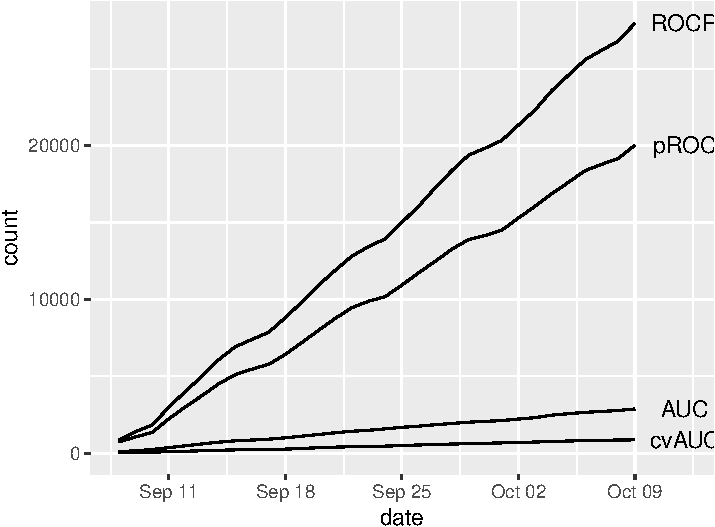
\includegraphics{index_files/figure-latex/unnamed-chunk-15-2} \end{center}

\end{CodeChunk}

\hypertarget{stata}{%
\subsection{Stata}\label{stata}}

\begin{CodeChunk}

\begin{CodeInput}
R> roctab x y
\end{CodeInput}


\begin{CodeOutput}
 . roctab x y

                      ROC                    -Asymptotic Normal--
           Obs       Area     Std. Err.      [95% Conf. Interval]
         --------------------------------------------------------
           169     0.6037       0.0379        0.52952     0.67793
\end{CodeOutput}
\end{CodeChunk}

We can also show that if we use simple Monte Carlo sampling, we can
estimate this true AUC, based on the definition above. Here, the
function \code{est.auc} samples \(10^{6}\) random samples from \(X_{1}\)
and \(X_{0}\), then calculates \(\hat{P}(X_{1} > X_{0})\):

\begin{CodeChunk}

\begin{CodeInput}
R> est.auc = function(x, y, n = 1000000) {
R+   x1 = x[y == 1] # sample x | y = 1
R+   x0 = x[y == 0] # sample x | y = 0
R+   c1 = sample(x1, size = n, replace = TRUE)
R+   c0 = sample(x0, size = n, replace = TRUE)
R+   auc.defn = mean(c1 > c0) # compare
R+   auc.wties = auc.defn + 1/2 * mean(c1 == c0) # compare
R+   return(c(auc.defn = auc.defn,
R+            auc.wties = auc.wties))
R+ }
R> sample.estauc = est.auc(x, y)
R> sample.estauc
\end{CodeInput}

\begin{CodeOutput}
 auc.defn auc.wties 
0.3646780 0.6039805 
\end{CodeOutput}
\end{CodeChunk}

\begin{CodeChunk}
\begin{figure}

{\centering 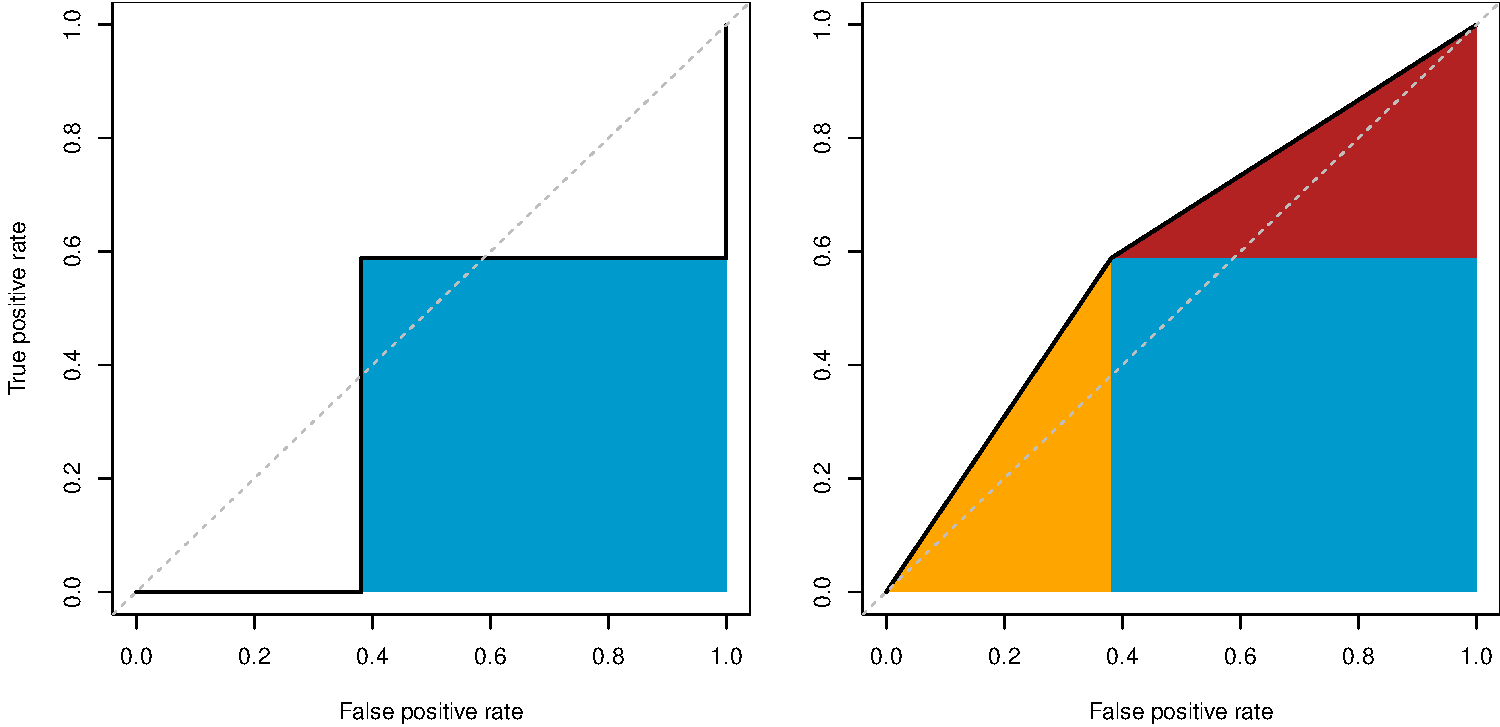
\includegraphics{index_files/figure-latex/unnamed-chunk-19-1} 

}

\caption[hey]{hey}\label{fig:unnamed-chunk-19}
\end{figure}
\end{CodeChunk}

One should note, that

\hypertarget{fawcett-example}{%
\subsection{Fawcett Example}\label{fawcett-example}}

\begin{CodeChunk}

\begin{CodeInput}
R> faw = data.frame(y = c(rep(TRUE, 6), rep(FALSE, 4)),
R+                  x = c(0.99999, 0.99999, 0.99993, 
R+                        0.99986, 0.99964, 0.99955, 
R+                        0.68139, 0.50961, 0.48880, 0.44951))
R> faw = faw %>% mutate(hyp = x > 0.5)
R> pred = prediction(predictions = faw[, "x"], labels = faw[, "y"])
R> par(mfrow = c(1, 2))
R> perf = performance(pred, "tpr", "fpr")
R> plot(perf)
R> abline(a = 0, b = 1)
R> plot(perf, type = "s")
R> abline(a = 0, b = 1)
\end{CodeInput}


\begin{center}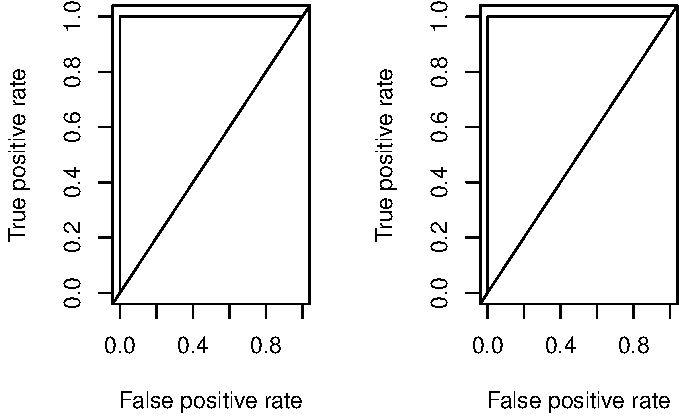
\includegraphics{index_files/figure-latex/fawcett-1} \end{center}


\begin{CodeInput}
R> auc.estimated = performance(pred, "auc")
R> yvalues(auc.estimated)
\end{CodeInput}

\begin{CodeOutput}
[1] 1
\end{CodeOutput}

\begin{CodeInput}
R> est.auc(x = faw[, "x"], y = faw[, "y"])
\end{CodeInput}

\begin{CodeOutput}
 auc.defn auc.wties 
        1         1 
\end{CodeOutput}
\end{CodeChunk}

\bibliography{binroc.bib}


\end{document}

